\section{Results}
\label{sec:results}
The experiment described in the experimental setup has been performed on the 938 EPUBs from the OAPEN Foundation dataset. This section will present the results that have come forth from this. In line with the latter two subquestions of this thesis, the subsections will cover the target error reduction and the original EPUB integrity, followed by a brief exposition of the computational overhead.

\subsection{Target error reduction}
The three target errors show a significant reduction after AccessiPub intervention. The results are visualized in Table \ref{table:targetreduction}. The largest reduction is for the \texttt{epub-pagelist-broken} error, which sees a complete 100\% reduction in errors after AccessiPub intervention. The \texttt{link-in-text-block} error is reduced by 97.7\%, and lastly, the \texttt{epub-pagelist-missing-pagebreak} error is reduced by 93.9\%. The total amount of target errors saw a reduction of 97.8\%, meaning an 83.6\% reduction in the total amount of errors in the dataset.


\subsubsection{Error reduction distribution}
To assess how AccessiPub performs over the whole dataset, the distribution of the reduction of errors is plotted in a histogram, visible in Figure \ref{figure:reduction}. The first bin of the histogram shows that many EPUBs do not have their errors reduced. A further analysis reveals that 438 EPUBs have zero error reduction. 429 of these EPUBs do not have any of the target errors, explaining the lack of error reduction, as these have not been processed by AccessiPub. This still leaves 9 EPUBs with target errors, that did not see any error reduction.
The histogram's far-right edge shows that many EPUBs still have their errors reduced significantly. Out of the 509 EPUBs with at least one of the target errors, 498 had all target errors eliminated. This large reduction in target errors meant a more than 90\% reduction in total errors for 344 EPUBs.

\begin{figure}[h]
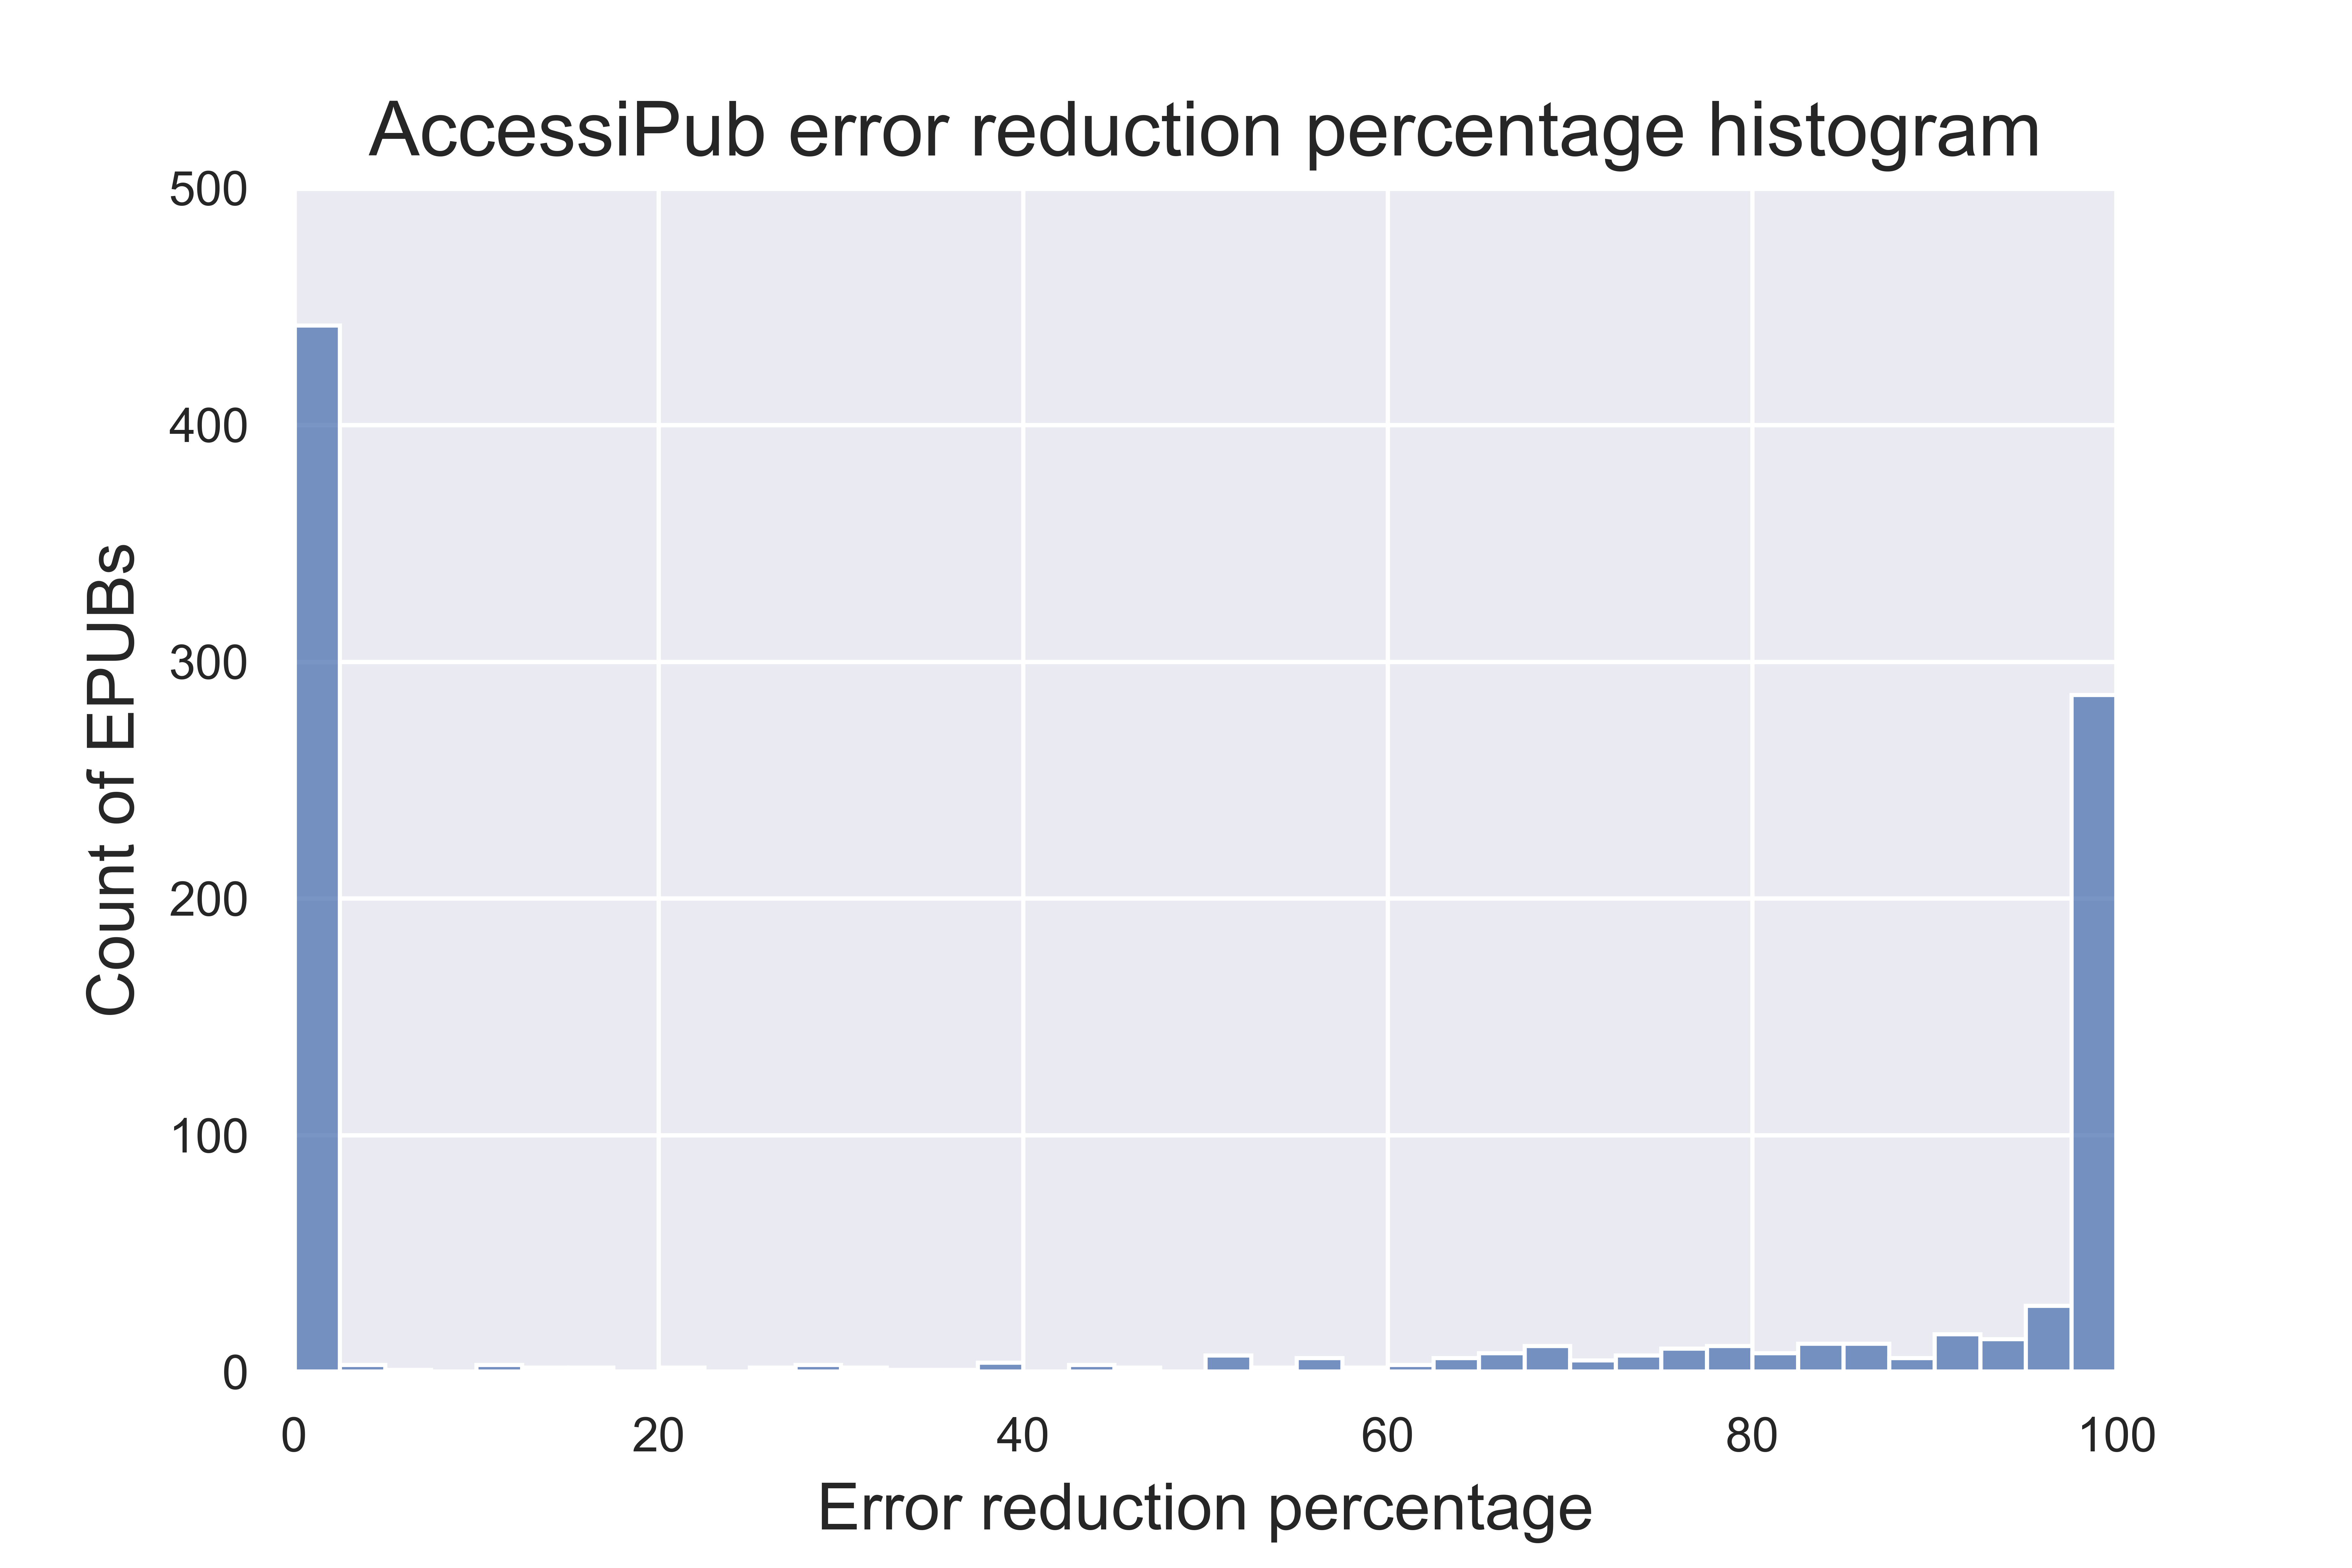
\includegraphics[width=0.48\textwidth,keepaspectratio]{media/images/fancy_reduction.png}
\caption{Distribution histogram of the number of EPUBs per error reduction percentage after AccessiPub intervention}
\centering
\label{figure:reduction}
\end{figure}

\subsubsection{Unprocessed EPUBs}
As the analysis of Figure \ref{figure:reduction} showed, 9 EPUBs with a target error did not see any reduction. A deeper dive into these 9 EPUBs shows the cause behind this. AccessiPub failed to process these EPUBs for three different reasons. 

Three EPUBs caused an error due to an incompliant file structure. The cover images were placed in the root folder of the EPUB, where only a mimetype file, a metadata folder, and a content folder should be present according to the EPUB3 standard. This caused a parsing error in the Ace checker, thus not being able to complete the evaluation, despite properly being processed by AccessiPub.

Two other EPUBs had a video represented in the EPUB manifest as a link to a cloud-hosted file. When EbookLib tried to disassemble this EPUB, it expected this video to be physically present in the content folder. However since it was hosted in the cloud, it was not found and EbookLib raised an error and was unable to continue. This is a known issue for the EbookLib developers\footnote{https://github.com/aerkalov/ebooklib/issues/281}.

The last four EPUBs that failed, did so because of a missing table of contents file. This missing table of contents caused EbookLib to generate an empty NCX file, since the generation of it depends on a table of contents. This empty NCX file caused a parsing error when EPUB reassembly was attempted. This is also a known issue for EbookLib\footnote{https://github.com/aerkalov/ebooklib/issues/130}.


\subsubsection{Incomplete target error reduction}
Out of the 509 EPUBs with at least one of the target errors, 498 EPUBs had all target errors eliminated. This means that 11 EPUBs did not have their target errors fully removed. 9 of these EPUBs were not processed as per the paragraph above, leaving 2 EPUBs with incomplete target error reduction. Further investigation reveals that both EPUBs were left with a singular \texttt{link-in-text-block} error. This appears to be falsely reported by Ace, as the link is visible as an accessible link when rendering in a browser. Evidence of this false error for both EPUBs can be found in Appendix \ref{sec:apx:first_appendix}. A GitHub issue for the Ace developers has been created\footnote{https://github.com/daisy/ace/issues/421}. This analysis allows us to report that, apart from unprocessed EPUBs and a bug in the Ace checker, AccessiPub was successful in removing all target errors.


\subsubsection{Statistical significance}
A paired samples t-test was performed to compare the number of errors in the full dataset before AccessiPub intervention and after AccessiPub intervention.
There was a significant difference in the amount of errors between the full dataset before AccessiPub intervention (M = 831.45, SD = 1112.11) and after AccessiPub intervention (M = 136.67, SD = 322.34); t(937) = 21.060, p = 6.461e-81.

% Additionally, a paired samples t-test was also performed on the target error dataset before AccessiPub intervention and after AccessiPub intervention.
% This evaluation also showed a significant difference in the amount of errors between the target error dataset before AccessiPub intervention (M = 1458.60, SD = 1173.41) and after AccessiPub intervention (M = 178.57, SD = 381.54); t(508) = 27.164, p = 5.000e-101.

% \begin{figure}[h]
% 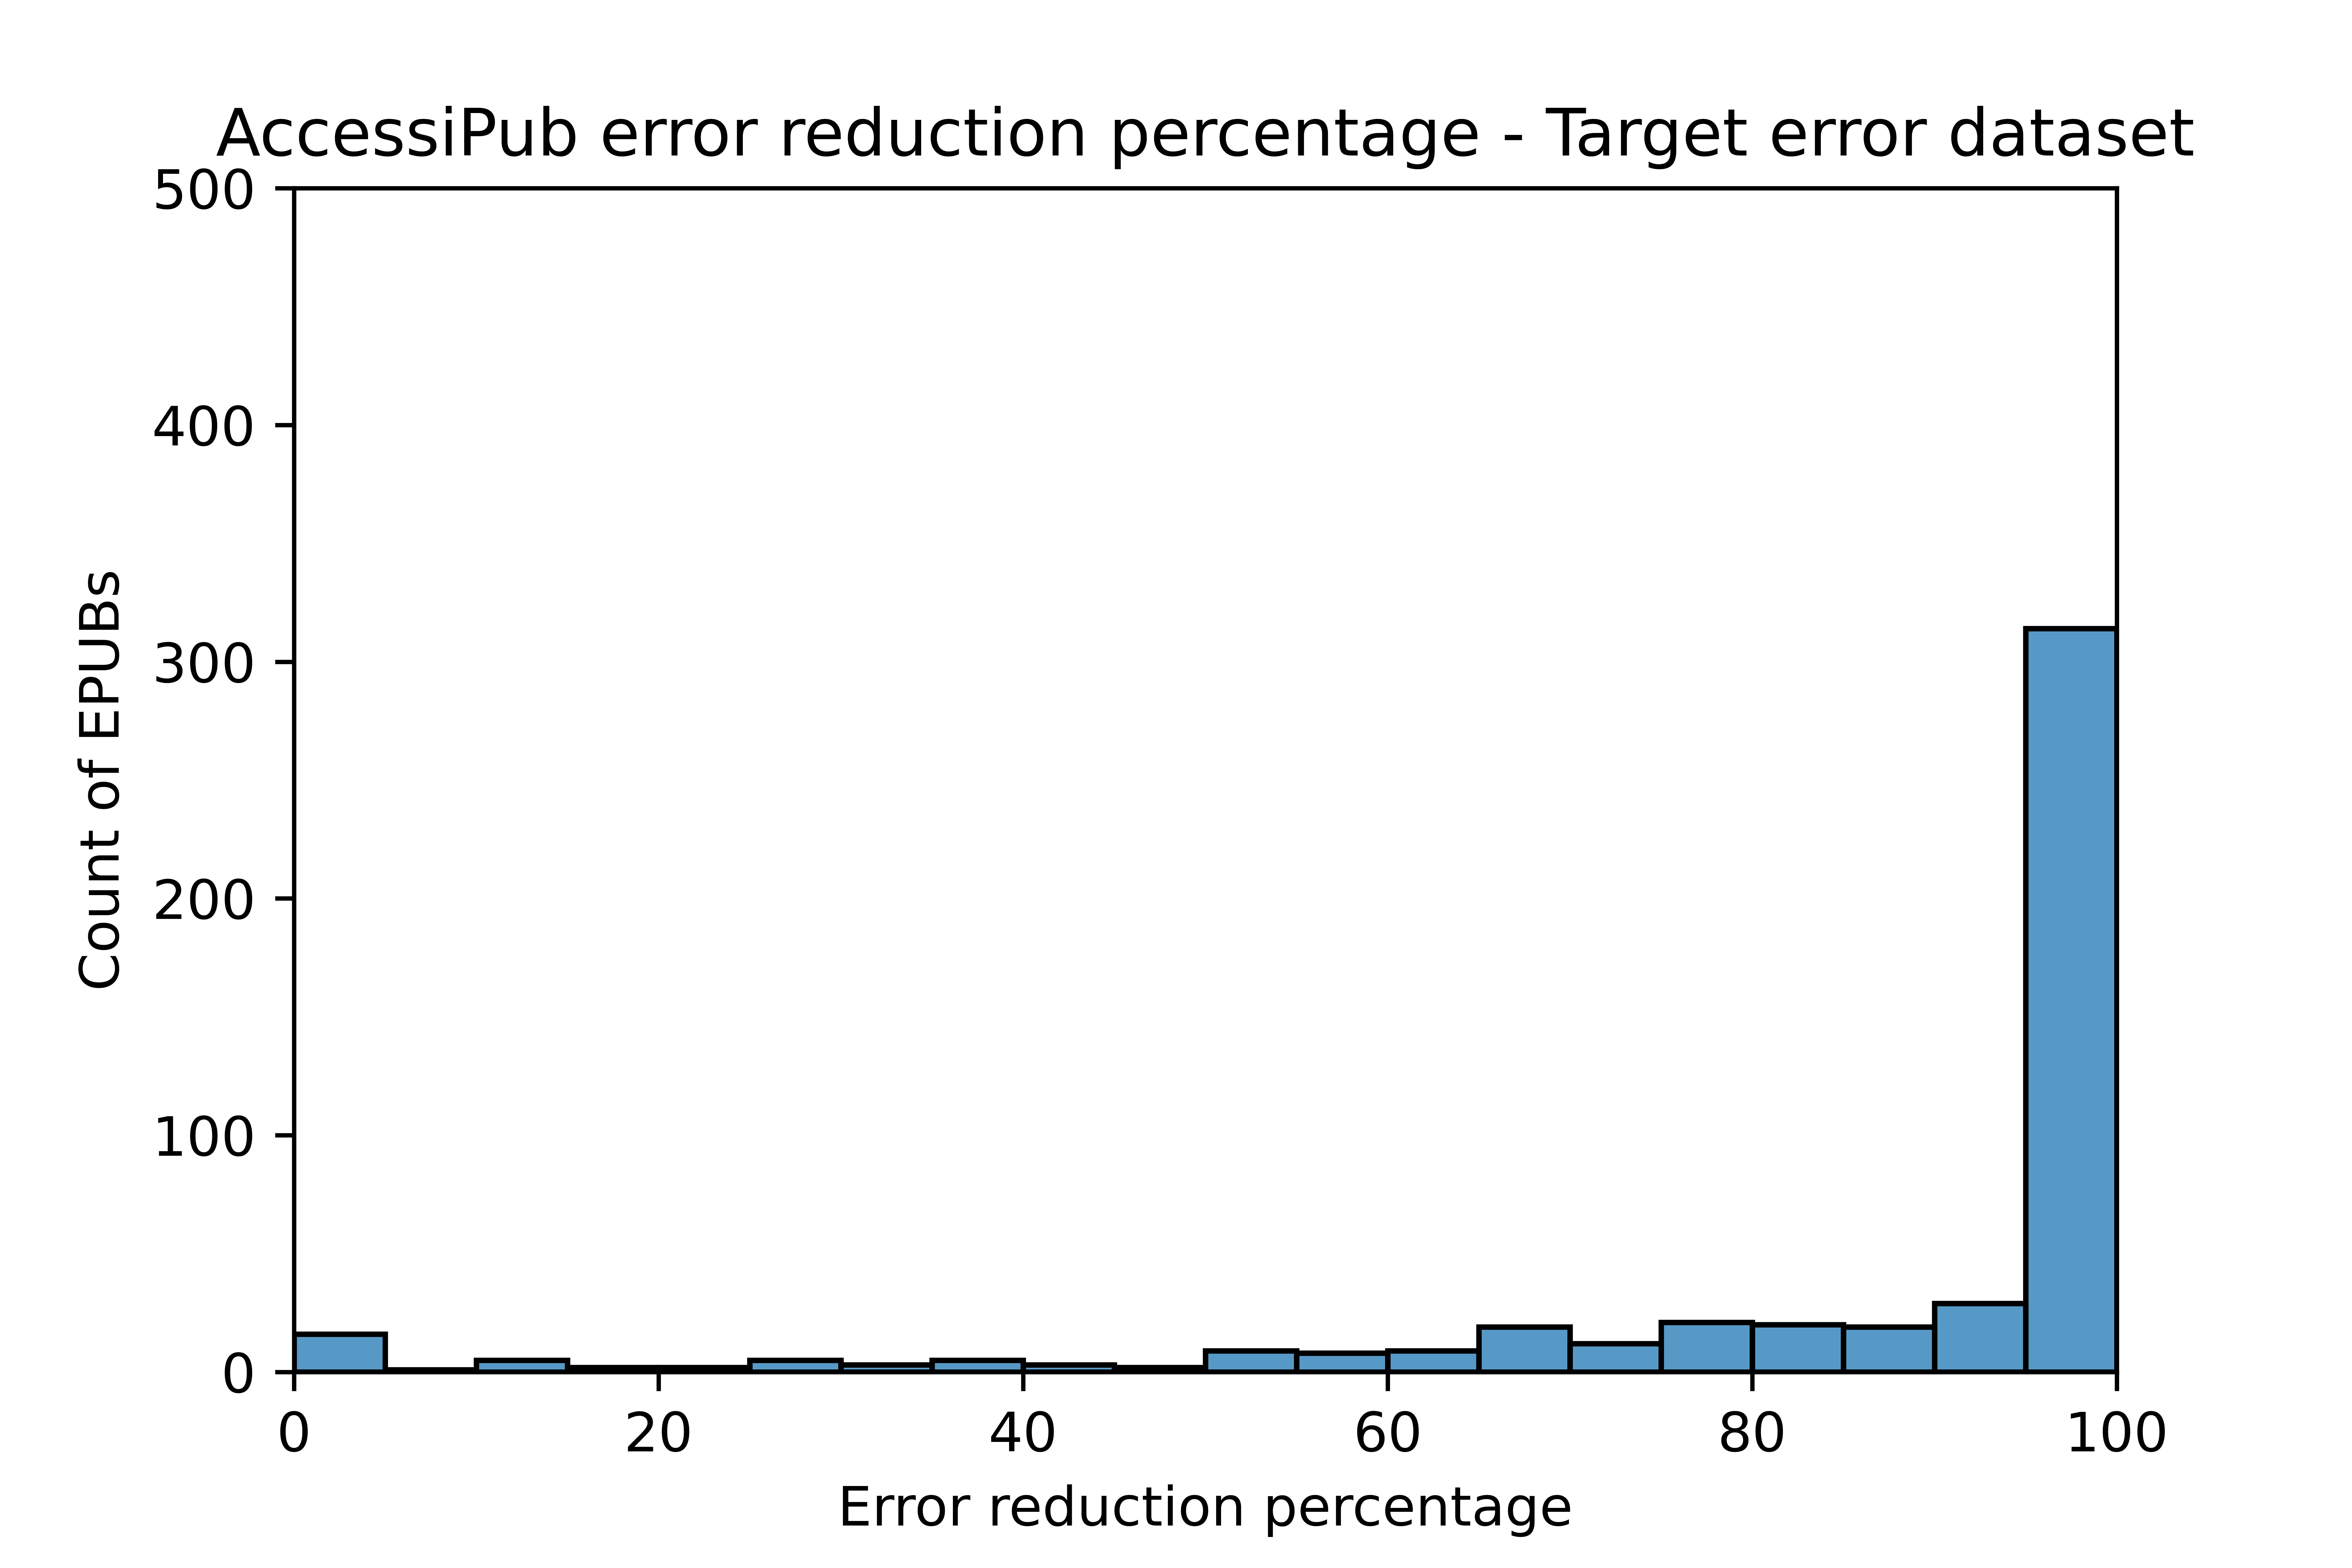
\includegraphics[width=0.4\textwidth,keepaspectratio]{media/images/TR_reduction.png}
% \caption{Distribution histogram of the reduction of errors per book after AccessiPub intervention on the data with the target errors}
% \centering
% \label{figure:tr_reduction}
% \end{figure}

\subsection{Original EPUB integrity}
The original EPUB integrity can be analyzed with the help of the visualization in Table \ref{table:integrity}. It shows that the overall amount of errors across all error classifications does not increase. A slight decrease is even seen for minor and moderate errors, which has to do with how EbookLib generates a new table of contents. The main decrease is still seen for the serious errors, since the target errors are all serious errors. 


\begin{table}[h!]
\small
\begin{center}
\begin{tabular}{ | c || c | c | c |} 
\hline
\textbf{Error classification} & \textbf{Before} & \textbf{After} & \textbf{\% Reduction} \\
\hline
Minor & 94,993 & 94,512 & -0.5\% \\
\hline
Moderate & 2,674 & 2,587 & -3.3\% \\
\hline
Serious & 682,133 & 30,996 & -95.5\% \\
\hline
Critical & 99 & 99 & 0\% \\
\hline
\hline
Total errors & 779,899 & 128,194 & -83.6\% \\
\hline
\end{tabular}
\end{center}
\normalsize
\caption{Overall error reduction per Ace error classification before and after AccessiPub intervention}
\label{table:integrity}
\end{table}

While the overall amount of errors did indeed not increase, certain individual errors did increase. This is visualized in Table \ref{table:errorincrease}. The first error describes that each HTML document must contain a non-empty \texttt{<title>} element. The second error describes a faulty order in the table of contents. The latter five errors all relate to missing metadata in the .opf file that describes an EPUB's accessibility characteristics. When taken all together, this increase in errors is very small. In total 18 errors are added to the grand total of 128,360 after AccessiPub intervention. 

\begin{table}[h!]
\small
\begin{center}
\begin{tabular}{ | c || c | c | c |} 
\hline
\textbf{Error type} & \textbf{Before} & \textbf{After} & \textbf{Increase} \\
\hline
document-title & 463 & 466 & 3 \\
\hline
epub-toc-order & 3 & 12 & 9 \\
\hline
metadata-accessibilityfeature & 637 & 639 & 2 \\
\hline
metadata-accessibilityhazard & 654 & 655 & 1 \\
\hline
metadata-accessibilitysummary & 645 & 646 & 1 \\
\hline
metadata-accessmode & 638 & 639 & 1 \\
\hline
metadata-accessmodesufficient & 638 & 639 & 1 \\
\hline
\end{tabular}
\end{center}
\normalsize
\caption{Error increase for certain error types before and after AccessiPub intervention}
\label{table:errorincrease}
\end{table}

The errors do indicate that the EPUB patching step has not gone without errors. The first error indicates that information inside the \texttt{<head>} tag has gone missing for three HTML documents across three separate EPUBs. The latter five errors point to the fact that the missing accessibility metadata in the .opf file was not correctly patched, either on one or two occasions. 

\subsection{Computational Overhead}
A short overview of the computational overhead can be found in Table \ref{table:computational_overhead}. The execution times were found using a laptop with an AMD Ryzen 5 4600U processor while the system consumed on average 500MB of RAM. The table shows that an average EPUB takes under 3 seconds to be fully processed by AccessiPub.


\begin{table}[h!]
\small
\begin{center}
\begin{tabular}{ | c | c |} 
\hline
\textbf{Task} & \textbf{Execution time} \\
\hline
EPUB disassembly & 140 ms \\
\hline
Error finding and fixing & 100 ms \\
\hline
EPUB reassembly & 420 ms \\
\hline
EPUB patching & 2050 ms \\
\hline
\end{tabular}
\end{center}
\normalsize
\caption{Computational overhead in milliseconds per AccessiPub task for an average single EPUB}
\label{table:computational_overhead}
\end{table}